% experiments.tex — DisPeD Experiments Section
% Requires: booktabs, multirow, graphicx, multicolumn (standard)

\section{Experiments}
\label{sec:experiments}

\subsection{Experimental Setup}
\label{sec:setup}

\paragraph{Datasets.}
We train on 250 Crescendo~\citep{russinovich2024crescendo} jailbreak conversations and 250 topic-anchored benign conversations, both generated via Qwen3-8B.
Topic anchoring ensures that benign conversations cover the same subject domains as jailbreak conversations and controls for topical confounds.
For out-of-distribution (OOD) evaluation, we generate 80 Foot-in-the-Door (FITD)~\citep{fitd2024} and 80 Deceptive Delight (DD)~\citep{deceptivedelight2024} conversations through a separate pipeline with no overlap in attack templates or strategies with the training data.
The in-distribution (IID) test set consists of 76 held-out Crescendo conversations (38 jailbreak, 38 benign).
To assess adversarial robustness, we paraphrase the IID test set to produce 76 perturbed samples with mean BERTScore of 0.92 and lexical overlap of 0.20, confirming that surface forms change substantially while semantics are preserved.

\paragraph{Baselines.}
We compare three detection methods.
\textbf{DisPeD} (ours): DeBERTa-v3-base~\citep{he2021deberta} fine-tuned with a multi-task objective combining 9-class persuasion strategy classification and binary jailbreak-intent classification (Section~\ref{sec:method}).
Turn-level [CLS] embeddings are aggregated via a bidirectional GRU (BiGRU) for conversation-level binary classification.
\textbf{Vanilla DeBERTa}: the identical pipeline with an unfine-tuned DeBERTa encoder.
This baseline isolates the effect of persuasion-aware fine-tuning.
\textbf{TF-IDF LR}: TF-IDF features over full conversation text with logistic regression, serving as a lexical baseline.
We additionally evaluate LLM-as-judge baselines in Section~\ref{sec:llm_judge}.

\paragraph{Metrics and implementation.}
We report F1 score for binary jailbreak detection at turn prefix lengths $K \in \{1, 2, 3, 5\}$ and on full conversations.
IID results report the mean and standard deviation across three random seeds (42, 123, 456); OOD results use seed 42.
Stage-1 fine-tuning uses a learning rate of $2 \times 10^{-5}$, batch size 16, and 4 epochs.
The multi-task loss weight $\alpha$ is set to 0.3.
The 9-class persuasion taxonomy is grounded in the Persuasion Attack Paradigm~\citep{zeng2024pap} and Cialdini's influence principles~\citep{cialdini2001influence}, with turn-level annotations produced by Qwen3-8B.
Stage-2 classification uses a two-layer MLP trained for 20 epochs over BiGRU-aggregated [CLS] embeddings.

%----------------------------------------------------------------------
\subsection{Cross-Attack Generalization}
\label{sec:cross_attack}

\begin{table*}[t]
\centering
\small
\caption{Cross-attack generalization (F1). All models trained on Crescendo conversations. IID results report 3-seed mean$\pm$std (seeds 42, 123, 456). OOD results use seed 42. $K$ denotes the number of conversation turns used for detection. Best per column per section in \textbf{bold}, second best \underline{underlined} (when three or more methods report values).}
\label{tab:main_results}
\begin{tabular}{@{}lccccc@{}}
\toprule
\textbf{Method} & $K$=1 & $K$=2 & $K$=3 & $K$=5 & Full \\
\midrule
\multicolumn{6}{l}{\textit{IID (Crescendo)}} \\[2pt]
DisPeD (ours) & \textbf{1.000$\pm$.000} & \textbf{1.000$\pm$.000} & \textbf{1.000$\pm$.000} & \textbf{1.000$\pm$.000} & \textbf{1.000$\pm$.000} \\
Vanilla DeBERTa & .968$\pm$.033 & .978$\pm$.016 & .987$\pm$.000 & \underline{.982$\pm$.014} & \textbf{1.000$\pm$.000} \\
TF-IDF LR & \textbf{1.000$\pm$.000} & \textbf{1.000$\pm$.000} & \textbf{1.000$\pm$.000} & \textbf{1.000$\pm$.000} & \textbf{1.000$\pm$.000} \\
\midrule
\multicolumn{6}{l}{\textit{OOD (Deceptive Delight)}} \\[2pt]
DisPeD (ours) & \textbf{1.000} & \textbf{.990} & \textbf{.990} & \textbf{1.000} & \textbf{1.000} \\
Vanilla DeBERTa & .575 & .438 & .360 & .311 & .284 \\
TF-IDF LR & -- & -- & -- & -- & \underline{.944} \\
\midrule
\multicolumn{6}{l}{\textit{OOD (FITD)}} \\[2pt]
DisPeD (ours) & \textbf{1.000} & \textbf{1.000} & -- & -- & \textbf{1.000} \\
Vanilla DeBERTa & \underline{.990} & \textbf{1.000} & -- & -- & \textbf{1.000} \\
TF-IDF LR & \textbf{1.000} & -- & -- & -- & \textbf{1.000} \\
\bottomrule
\end{tabular}
\end{table*}

\begin{figure}[t]
\centering
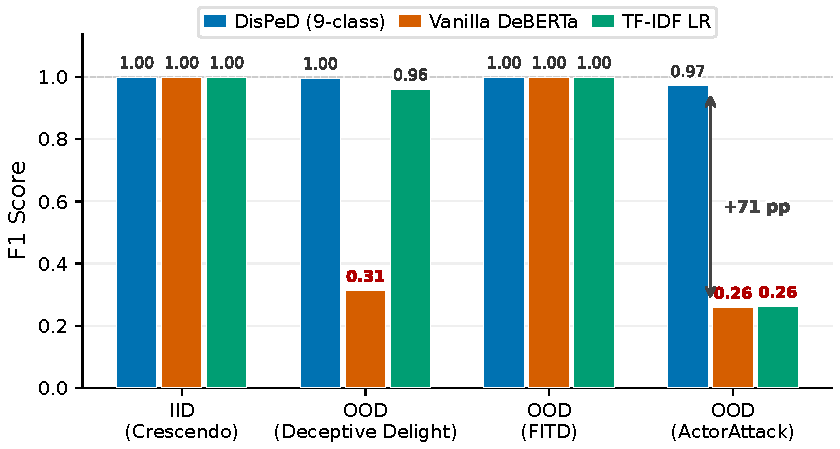
\includegraphics[width=\columnwidth]{figures/paper/fig2_cross_attack_bar.pdf}
\caption{Cross-attack generalization at full conversation length. Vanilla DeBERTa collapses on unseen Deceptive Delight (F1 = 0.284) while DisPeD maintains F1 = 1.000. TF-IDF LR achieves 0.944 on DD, reflecting inherent lexical separability.}
\label{fig:cross_attack}
\end{figure}

Persuasion-aware fine-tuning enables robust detection of unseen attack types where vanilla semantic embeddings collapse.
Table~\ref{tab:main_results} presents F1 scores across three test conditions: IID Crescendo, OOD Deceptive Delight, and OOD FITD.
Figure~\ref{fig:cross_attack} provides a visual comparison at full conversation length.

\paragraph{IID performance.}
All three methods achieve near-perfect F1 on in-distribution Crescendo test data.
TF-IDF LR and DisPeD both reach F1 = 1.000 at every prefix length, and Vanilla DeBERTa ranges from 0.968 to 1.000.
This ceiling effect reflects an inherent lexical separability between persuasive jailbreak and general benign conversations: even bag-of-words features suffice when the test distribution matches training.
The IID results confirm that persuasion-aware fine-tuning does not sacrifice in-distribution accuracy.
Vanilla DeBERTa shows the most variance at early prefixes ($K$=1: std=0.033), where fewer turns provide less signal for generic embeddings.
DisPeD achieves zero variance (std=0.000) across all prefix lengths, reflecting stable representations even with limited context.

\paragraph{OOD: Deceptive Delight.}
The DD evaluation reveals the central finding of this paper.
Vanilla DeBERTa, the natural approach of encoding turns with a generic pretrained model, collapses to F1 = 0.284 on full DD conversations despite reaching 1.000 on IID data from the same pipeline.
The degradation worsens as more turns are observed: F1 drops from 0.575 at $K$=1 to 0.284 at Full.
This counterintuitive pattern is consistent with prior work showing that multi-turn attack turns are designed to remain in a ``benign'' embedding region~\citep{bullwinkel2025repeng}: each additional DD turn supplies more misleading ``benign'' evidence, pushing the model toward incorrect predictions rather than helping it detect the attack.
DisPeD maintains F1 $\geq$ 0.990 at every prefix length, including near-perfect early detection at $K$=1 (F1 = 1.000) and $K$=2 (F1 = 0.990).
The gap over Vanilla DeBERTa ranges from +42 percentage points at $K$=1 to +72 percentage points at Full.
Early detection is particularly important for deployment: at $K$=2, DisPeD detects attacks after just two turns (F1 = 0.990) while Vanilla DeBERTa has already dropped to 0.438.

TF-IDF LR achieves F1 = 0.944 on full DD conversations, which confirms substantial lexical separability even across attack families.
We acknowledge this result openly: the primary contribution of DisPeD over TF-IDF is not raw detection performance but rather three complementary advantages.
First, DisPeD bridges the representation-level gap that vanilla semantic embeddings cannot (+72 percentage points on DD), validating persuasion-aware fine-tuning as the mechanism for cross-attack generalization.
Second, DisPeD achieves zero degradation under adversarial perturbation (Section~\ref{sec:perturbation}).
Third, DisPeD provides interpretable strategy trajectories for detection decisions (Section~\ref{sec:strategy}).

\paragraph{OOD: FITD.}
FITD conversations are easier to detect across all methods.
DisPeD and Vanilla DeBERTa both reach F1 $\geq$ 0.990 at all evaluated prefixes, and TF-IDF LR achieves 1.000 on $K$=1 and full conversations.
The limited differentiation on FITD suggests this attack family shares more surface-level features with the Crescendo training data than DD does, reducing the cross-attack generalization challenge.

%----------------------------------------------------------------------
\subsection{Ablation Study}
\label{sec:ablation}

\begin{table}[t]
\centering
\small
\caption{Ablation study on OOD Deceptive Delight and IID. All variants trained on Crescendo. The persuasion fine-tuning process is the critical factor; label granularity and temporal modeling are not.}
\label{tab:ablation}
\begin{tabular}{@{}lccc@{}}
\toprule
\textbf{Variant} & DD-Full & DD-$K$=2 & IID-Full \\
\midrule
DisPeD (9-class) & \textbf{1.000} & \textbf{.990} & 1.000 \\
Scrambled labels & .990 & .981 & 1.000 \\
Binary (2-class) & .990 & .981 & 1.000 \\
Mean pooling & \textbf{1.000} & \textbf{.990} & 1.000 \\
\midrule
Vanilla DeBERTa & .284 & .438 & 1.000 \\
\bottomrule
\end{tabular}
\end{table}

The fine-tuning process on persuasion-related text, not specific label assignments, is what drives cross-attack generalization.
Table~\ref{tab:ablation} reports DD-OOD and IID F1 for several model variants, grouped into fine-tuned variants (above the mid-rule) and the unfine-tuned baseline (below).

\paragraph{Label granularity.}
Replacing the 9-class persuasion taxonomy with randomly scrambled labels reduces DD-Full F1 from 1.000 to 0.990, a gap of just 1 percentage point.
Collapsing the taxonomy to binary (persuasion-present vs.\ absent) yields the same 0.990.
Both variants remain far above the vanilla baseline (F1 = 0.284), a gap exceeding 70 percentage points.
These results confirm that the encoder learns useful pragmatic features from exposure to persuasion-domain text during fine-tuning, regardless of whether strategy labels are correct, coarse, or random.
The data domain matters more than the specific supervision signal~\citep{gururangan2020dontstop}.
In our setting, multi-task fine-tuning on persuasion-related conversations teaches the encoder to attend to pragmatic features (e.g., implicit requests, escalation cues, rapport-building patterns) that transfer across attack types.
The 9-class taxonomy provides interpretability through strategy trajectory analysis (Section~\ref{sec:strategy}) rather than a detection advantage over coarser alternatives.
From a practical standpoint, this result lowers the annotation barrier: coarse or imperfect persuasion labels suffice for training an effective cross-attack detector.

\paragraph{Temporal modeling.}
Replacing BiGRU with orderless mean pooling over the [CLS] sequence yields DD-Full F1 = 1.000, matching the BiGRU default.
This equivalence confirms that the model detects persuasion presence in individual turns rather than relying on the temporal ordering of strategies across the conversation.
BiGRU is the default aggregator in all other experiments.

\paragraph{Fine-tuning as the critical factor.}
The most informative comparison spans all ablation rows.
Every variant that includes persuasion-domain fine-tuning achieves DD-Full F1 $\geq$ 0.990, while Vanilla DeBERTa collapses to 0.284.
All fine-tuned variants also maintain IID-Full F1 = 1.000.
This 70+ percentage point gap on OOD data establishes that persuasion-aware fine-tuning is both necessary and sufficient for cross-attack generalization; architecture choices and label granularity are secondary factors.
We also evaluated an $\alpha=0$ variant (persuasion strategy classification only, no intent task), which achieves IID-Full F1 = 1.000. OOD evaluation was not conducted for this variant, but the IID result confirms that the persuasion task alone suffices for in-distribution detection. The intent head provides a complementary training signal but is not required when the persuasion task drives representation learning.

\paragraph{Domain-adaptive controls.}
The scrambled-label result raises a question: does the encoder benefit from persuasion-specific pragmatic features, or from domain adaptation on conversational text more broadly? To isolate this, we are conducting two control experiments. The first replaces the persuasion strategy head with sentiment classification on the same training data, testing whether any auxiliary task on in-domain text suffices. The second applies masked language modeling (MLM) on the training conversations without any classification head, testing whether unsupervised domain adaptation alone accounts for the OOD gains. \texttt{[PENDING: plan\_016/017 domain-adaptive control results]}

%----------------------------------------------------------------------
\subsection{Robustness Under Adversarial Perturbation}
\label{sec:perturbation}

\begin{table}[t]
\centering
\small
\caption{Robustness under adversarial paraphrasing (IID test set, full conversations). Perturbed set preserves semantics (BERTScore 0.92) while altering surface forms (lexical overlap 0.20). $\Delta$: degradation in percentage points.}
\label{tab:perturbation}
\begin{tabular}{@{}lccc@{}}
\toprule
\textbf{Method} & Original & Perturbed & $\Delta$ (pp) \\
\midrule
DisPeD (ours) & \textbf{1.000} & \textbf{1.000} & \textbf{0.0} \\
Vanilla DeBERTa & 1.000 & .882 & $-$11.8 \\
TF-IDF LR & 1.000 & \underline{.987} & \underline{$-$1.3} \\
\bottomrule
\end{tabular}
\end{table}

DisPeD maintains perfect detection under adversarial paraphrasing while both baselines degrade.
Table~\ref{tab:perturbation} reports F1 on the original and perturbed IID test sets (76 samples each).
The perturbed set was constructed via automated paraphrasing that preserves semantic content (BERTScore 0.92) while substantially altering surface forms (lexical overlap 0.20).

DisPeD achieves F1 = 1.000 on both original and perturbed data, with zero degradation.
Vanilla DeBERTa drops from 1.000 to 0.882, a loss of 11.8 percentage points, consistent with its reliance on surface-level features from the unfine-tuned encoder.
TF-IDF LR shows a smaller but measurable decline from 1.000 to 0.987 (1.3 percentage points).
The ordering follows the expected robustness hierarchy: features learned through persuasion-aware fine-tuning capture pragmatic patterns that are invariant to surface rephrasing, while generic embeddings and lexical features are more sensitive to word-level changes.
Combined with the cross-attack results in Table~\ref{tab:main_results}, the perturbation evaluation confirms that persuasion-aware fine-tuning produces representations robust to both unseen attack types and adversarial surface variation.
The zero-degradation result is particularly relevant for deployment scenarios where attackers may attempt to evade detection through paraphrasing or style transfer~\citep{nasr2025attackermovessecond}.
While our perturbation evaluation uses automated paraphrasing rather than adversary-crafted evasion, the 11.8 percentage point degradation of Vanilla DeBERTa under even this moderate perturbation suggests that unfine-tuned representations would be fragile against more targeted adaptive attacks.

%----------------------------------------------------------------------
\subsection{LLM-as-Judge Baseline}
\label{sec:llm_judge}

\begin{table}[t]
\centering
\small
\caption{LLM-as-judge zero-shot Crescendo detection (IID test set). F1 values exclude unparseable responses and therefore represent upper bounds.$^{\dagger}$Unparseable rate increases with context length: 30\% at $K$=2 to 47\% at Full.}
\label{tab:llm_judge}
\begin{tabular}{@{}lccccr@{}}
\toprule
\textbf{Method} & $K$=2 & $K$=3 & $K$=5 & Full & Unparse. \\
\midrule
GPT-5.5 & .191 & .273 & .449 & .383 & 30--47\%$^{\dagger}$ \\
Qwen3-8B & .000 & .051 & .146 & .100 & 0\% \\
\midrule
DisPeD (ours) & \textbf{1.000} & \textbf{1.000} & \textbf{1.000} & \textbf{1.000} & 0\% \\
\bottomrule
\end{tabular}
\end{table}

Frontier language models fail at multi-turn jailbreak detection even when given full conversation context.
Table~\ref{tab:llm_judge} reports zero-shot detection performance for GPT-5.5 and Qwen3-8B on the IID Crescendo test set, where both models are prompted to classify each conversation as jailbreak or benign.

GPT-5.5 achieves precision of 1.0 at all turn prefixes but recall ranges from only 0.105 to 0.290, resulting in F1 of 0.191 at $K$=2 and 0.449 at $K$=5.
A substantial fraction of GPT-5.5 responses are unparseable: the rate increases from 30\% at $K$=2 to 47\% on full conversations.
The F1 values in Table~\ref{tab:llm_judge} exclude unparseable responses and therefore represent upper bounds on actual performance.
Full-conversation F1 (0.383) is lower than $K$=5 F1 (0.449) because the unparseable rate grows with context length, not because the model classifies worse on parsed responses.
The high precision but low recall pattern suggests that GPT-5.5 is deceived by Crescendo's surface educational framing: when the model does commit to a classification, it correctly identifies jailbreaks, but the majority of attacks go undetected.

Qwen3-8B performs worse across all prefixes, with F1 from 0.000 at $K$=2 to 0.100 on full conversations, and produces no unparseable responses.
The failure of both a frontier commercial model and an open-weight model highlights a fundamental limitation of content-level reasoning for this task.
Multi-turn jailbreak attacks distribute adversarial intent across individually benign turns~\citep{russinovich2024crescendo,li2024mhj}, and each turn maintains surface-level coherence with an innocuous cover topic.
An LLM analyzing conversation content sees a plausible discussion and lacks the pragmatic signal to recognize the underlying persuasion process.
DisPeD's learned persuasion features capture this pragmatic layer at a fraction of the inference cost of a frontier LLM, without requiring the conversation content to contain explicit harmful requests.

%----------------------------------------------------------------------
\subsection{Strategy Trajectory Analysis}
\label{sec:strategy}

\begin{figure*}[t]
\centering
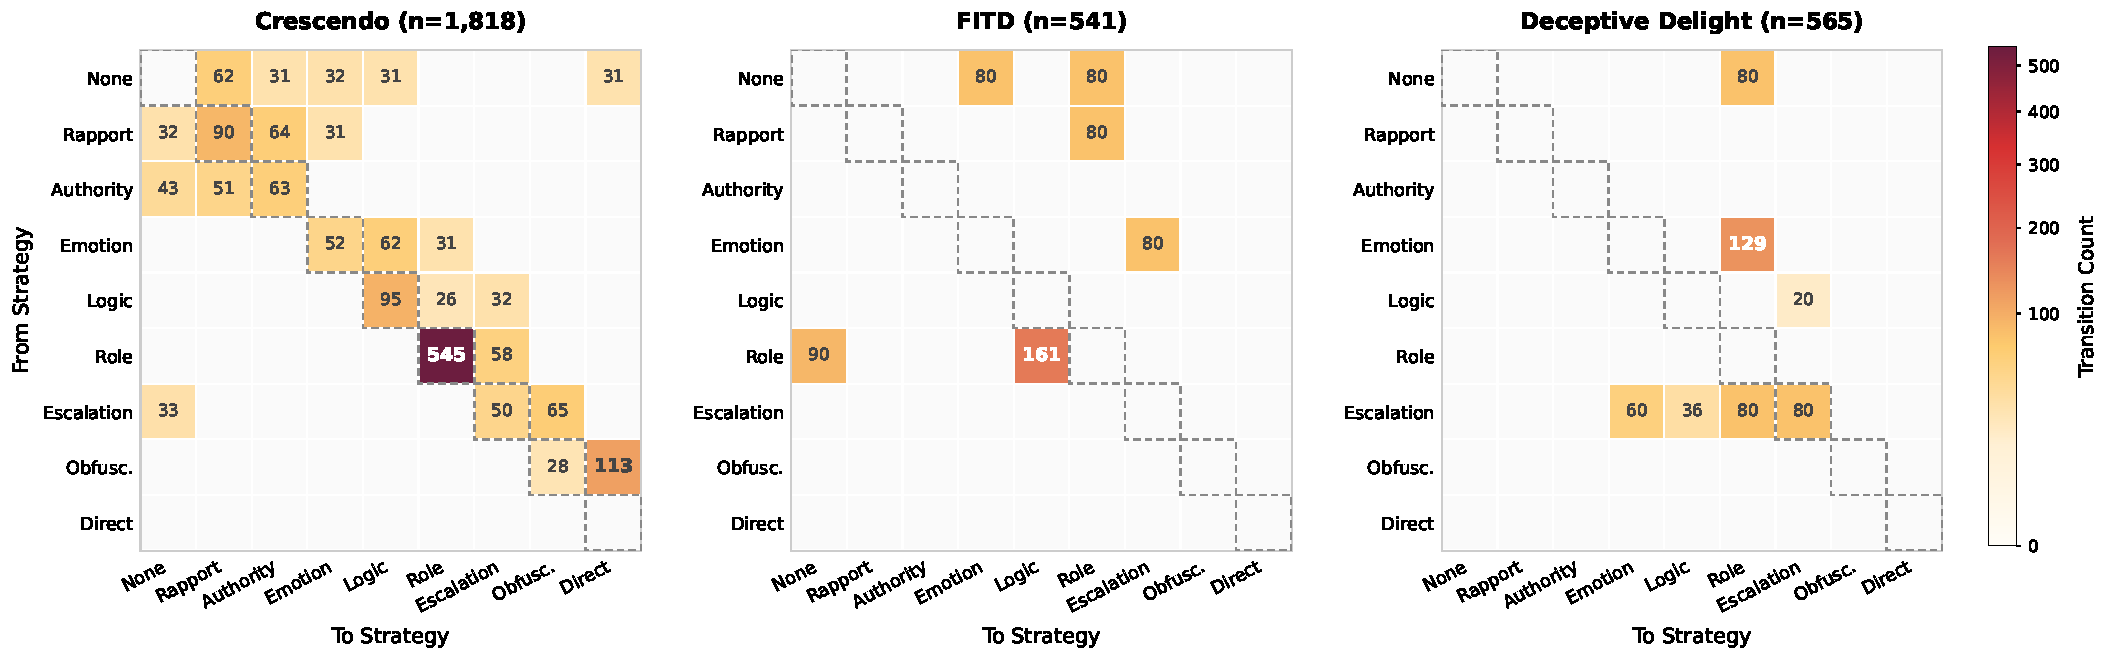
\includegraphics[width=\textwidth]{figures/paper/fig3_strategy_heatmap.pdf}
\caption{Persuasion strategy transition count matrices for three attack types, based on ground-truth intended strategy labels from the dataset generation pipeline. Color intensity reflects transition count on a symmetric log scale; white cells indicate zero transitions. Crescendo exhibits broad coverage across all strategy categories, while FITD and DD concentrate transitions in smaller subsets.}
\label{fig:strategy_heatmap}
\end{figure*}

Different multi-turn attack types produce distinct persuasion strategy transition patterns that provide native interpretability for detection decisions.
Figure~\ref{fig:strategy_heatmap} shows transition count matrices based on ground-truth intended strategy labels for three attack types.

Crescendo conversations exhibit broad transition coverage across all strategy categories, with 1,818 total transitions.
The highest concentration appears in Role Assignment self-transitions (545), with substantial activity across Emotional Manipulation, Logical Reframing, and Authority Appeal transitions.
This diverse pattern reflects Crescendo's design: each turn draws from a wide repertoire of strategies while incrementally shifting toward more aggressive persuasion.

FITD conversations show a markedly sparser pattern with 541 transitions concentrated in 4 active source strategies.
Role$\to$Obfuscation (161) is the dominant transition, consistent with FITD's structure of securing initial compliance through role assignment before obscuring the escalation path.

DD conversations span 5 active source strategies across 565 transitions.
Emotion$\to$Obfuscation (129) is the dominant transition, consistent with DD's hybrid design of embedding harmful content within emotionally engaging and distracting contexts~\citep{deceptivedelight2024}.

These trajectory signatures serve two purposes.
For practitioners, they provide human-interpretable explanations for detection decisions: a security analyst can inspect the strategy sequence to understand why a conversation was flagged.
For the research question, the diversity of trajectories across attack families confirms that persuasion-aware fine-tuning captures generalizable pragmatic structure rather than memorizing surface patterns from a single attack type.
We emphasize that strategy trajectories are an interpretability contribution, not a detection mechanism: the ablation in Section~\ref{sec:ablation} shows that replacing BiGRU with mean pooling (which discards turn order) yields identical performance, so DisPeD detects persuasion presence per turn rather than relying on temporal trajectory patterns.
